\section{Diskussion}
\label{sec:diskussion}

\subsection{Abweichungen}

Die Schallgeschwindigkeit in Acryl wurde in \autoref{sec:auswertung:schallgeschwindigkeit}
zu $\SI{2763.38(1046)}{\meter\per\second}$ bestimmt.
Ausgehend vom \hyperref[tab:vorbereitung]{Literaturwert} $\SI{2730}{\meter\per\second}$
entspricht das einer Abweichung von $\SI{33.38}{\meter\per\second}$ beziehungsweise $\SI{1.22}{\percent}$.
Es ist jedoch anzumerken,
dass sich diese Angabe auch von Quelle zu Quelle unterscheidet.

\autoref{fig:plt:visualization_bars} stellt die Abweichungen
von Schieblehre und Ultraschall aus \autoref{fig:plt:visualization}
nochmals anders dar.
Der aus den Messungen mit Schieblehre berechenbare Mittelpunkt der jeweiligen Fehlstelle wird zentriert,
und sämtliche Messungen werden relativ zu diesem geplottet.
Weil ein Messwert für \textbf{4} fehlt, ist dort kein Balken für die Ultraschall-Messung eingezeichnet.

\begin{figure}[H]
  \centering
  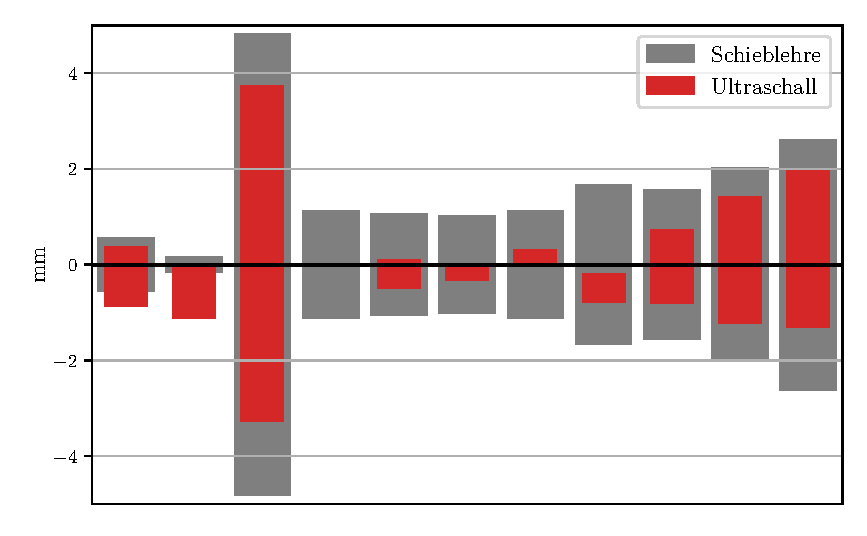
\includegraphics[width=\textwidth]{build/plt/visualization_bars.pdf}
  \caption{Visualisierung der Unterschiede der Messungen mit Schieblehre bzw. Ultraschall.}
  \label{fig:plt:visualization_bars}
\end{figure}

Insgesamt handelt es sich offenbar um sinnvolle Messwerte,
welche jedoch fast immer etwas zu große Distanzen angeben,
beziehungsweise umgerechnet eine kleinere als die mit der Schieblehre gemessene Lochgröße ergeben.
Daher liegt die Vermutung nahe,
dass ein systematischer Fehler vorliegt.

Mangels zuverlässiger Literaturwerte wird auf einen Vergleich der experimentell bestimmten Schallgeschwindigkeit in Acryl verzichtet.
Es lässt sich jedoch sagen,
dass die Abweichung des bestimmten Wertes mit $\pm \SI{10.46}{\meter\per\second}$ klein ausfällt.

Zum \hyperref[sec:auswertung:augenmodell]{Augenmodell} liegen ebenfalls keine Referenzwerte vor.

\subsection{Mögliche Fehlerquellen}

% Die zuvor besprochenen Abweichungen in der Messung der Distanz von Fehlstellen
% hängen möglicherweise mit der Beschaffenheit dieser zusammen.
% Sie sind nämlich rund… Joa…

% Der in \autoref{sec:auswertung:absorptionskoeffizient} bestimmte Absorptionskoeffizient $\alpha$ weicht,
% wie zuvor gezeigt, stark vom Literaturwert ab.
% → Aber welcher Literaturwert? Steht nur in irgendeinem Altprotokoll…

Sofern für die Schallgeschwindigkeit signifikante Abweichungen festzustellen sind,
ist eine wahrscheinliche Erklärung,
dass die Amplitude des Echos nicht nur von der Eindringtiefe,
sondern aufgrund der endlichen Breite der Schallwelle und der Sonde
auch von der Größe der Fehlstelle abhängt.
Da die Lochgröße von \textbf{4} bis \textbf{11} stets zunimmt,
ist nicht damit zu rechnen, dass sich dieser Effekt kompensiert.

Das Vermessen des Augenmodells war dadurch erschwert,
dass das resultierende Spektrum empfindlich von der Positionierung der Ultraschallsonde abhing.
Die Position der Peaks in der Zeit-Dimension sollte dadurch jedoch nur unwesentlich beeinflusst worden sein.

Beim Vermessen des Acrylblocks trat hingegen das Problem auf,
dass sich die Sonde nicht präzise über die Oberfläche bewegen ließ,
da sie aufgrund des verwendeten bidestillierten Wassers als Kontaktmittel
daran haftete.
Dadurch wurden Maxima weniger genau getroffen.
Beim Augenmodell wurde hingegen Ultraschallgel verwendet,
welches deutlich bessere Gleiteigenschaften besitzt.

% +++ Ich habe keine Ahnung… ↓
% Ein systematischer Fehler könnte weiterhin dadurch zustande kommen,
% dass das Piezo-Kristall der Ultraschallsonde nicht direkt auf dem Probekörper aufliegt:
% Einerseits gibt es eine "Plastik-Kappe",
% andererseits ist (insbesondere bei der Verwendung von Kontaktmittel) nicht gewährleistet,
% dass Sonde und Probe direkt in Kontakt sind.
% Durch leichtes Variieren des Druckes ließen sich tatsächlich kleine Änderungen beobachten.
% Diese Distanz müsste von den Messwerten zuerst subtrahiert werden.
% Es wird angenommen, dass dies von der Messapparatur oder dem Messprogramm bereits berücksichtigt wird,
% dazu liegen jedoch keine Informationen vor.
% +++ Ich habe keine Ahnung… ↑
